\documentclass{anstrans}
%%%%%%%%%%%%%%%%%%%%%%%%%%%%%%%%%%%
\title{An Improved ANS Transaction Template}
\author{Baptiste Mouginot,$^{*}$ Kathie Mummah,$^{*}$ Paul P.H. Wilson$^{*}$}

\institute{
$^{*}$University of Wisconsin-Madison, WI
}

\email{mouginot@wisc.edu \and mummah@wisc.edu \and paul.wilson@wisc.edu}

% Optional disclaimer: remove this command to hide
% \disclaimer{Notice: this manuscript is a work of fiction. Any resemblance to
% actual articles, living or dead, is purely coincidental.}

%%%% packages and definitions (optional)
\usepackage{graphicx} % allows inclusion of graphics
\usepackage{booktabs} % nice rules (thick lines) for tables
\usepackage{microtype} % improves typography for PDF

\newcommand{\SN}{S$_N$}
\renewcommand{\vec}[1]{\bm{#1}} %vector is bold italic
\newcommand{\vd}{\bm{\cdot}} % slightly bold vector dot
\newcommand{\grad}{\vec{\nabla}} % gradient
\newcommand{\ud}{\mathop{}\!\mathrm{d}} % upright derivative symbol

\begin{document}
%%%%%%%%%%%%%%%%%%%%%%%%%%%%%%%%%%%%%%%%%%%%%%%%%%%%%%%%%%%%%%%%%%%%%%%%%%%%%%%%
\section{Introduction}




Some text for introduction etc\ldots
Some text for introduction etc\ldots
Some text for introduction etc\ldots
Some text for introduction etc\ldots
Some text for introduction etc\ldots
Some text for introduction etc\ldots
Some text for introduction etc\ldots
Some text for introduction etc\ldots
Some text for introduction etc\ldots
Some text for introduction etc\ldots
Some text for introduction etc\ldots
Some text for introduction etc\ldots
Some text for introduction etc\ldots
Some text for introduction etc\ldots
Some text for introduction etc\ldots
Some text for introduction etc\ldots
Some text for introduction etc\ldots
Some text for introduction etc\ldots
Some text for introduction etc\ldots
Some text for introduction etc\ldots
Some text for introduction etc\ldots
Some text for introduction etc\ldots
Some text for introduction etc\ldots
Some text for introduction etc\ldots


%%%%%%%%%%%%%%%%%%%%%%%%%%%%%%%%%%%%%%%%%%%%%%%%%%%%%%%%%%%%%%%%%%%%%%%%%%%%%%%%
\section{Theory}



Some text for introduction etc\ldots
Some text for introduction etc\ldots
Some text for introduction etc\ldots
Some text for introduction etc\ldots
Some text for introduction etc\ldots
Some text for introduction etc\ldots
Some text for introduction etc\ldots
Some text for introduction etc\ldots
Some text for introduction etc\ldots
Some text for introduction etc\ldots
Some text for introduction etc\ldots
Some text for introduction etc\ldots
Some text for introduction etc\ldots
Some text for introduction etc\ldots
Some text for introduction etc\ldots
Some text for introduction etc\ldots


\section{Cascade Enrich Construction}
\subsection{Centrifuge properties}
In the present work, the analytical solution by R\"aetz \cite{ref} of the
differential equation for the gas centrifuge as described in \cite{Glaser2008}
is used. The different parameter of the centrifuges, such as average temperature
of the gas, rotation speed, height, feed flow rate, diameter, pressure ratio,
countercurent ratio, efficiency have been choosen to match the cascade design
describe in \cite{glaser2008} and \cite{Walker2017} using P-1 centrifuges and
repect the JCPOA aggrement.


\subsection{Cascade Design}

The cascade build as an ideal cascade, taht is to day, $\alpha =\beta = const$
for all stage of the cascade, where $\alpha$ and $\beta$ respectively represent
the feed to product and the feed to tail enrichment factors. 
$\alpha$ can be expressed as a function of the feed rate $F$, $\delta U(\theta)$ and $\theta$,
and $\beta$ as a function of $alpha$ and $\theta$: 
\begin{subequations} \label{eqs:alphabeta}
    \begin{equation} \label{eq:alpha}
    \alpha = \sqrt{\frac{2\delta U}{F} \frac{1-\theta}{\theta}}+1
\end{equation}
\\
\begin{equation}\label{eq:beta}
    \beta = R 
              \dfrac{1 - \dfrac{N - \theta \dfrac{\alpha R}{1+\alpha R}}{1 - \theta}}
                   {\dfrac{N - \theta \dfrac{\alpha R}{1+\alpha R}}{1 - \theta}} 
\end{equation}
\end{subequations}

From equation \eqref{eq:alpha} and \eqref{eq:beta} it is possible to determine the cut value
(all other centrifuge parameters been fixed) allowing the have $\alpha=\beta$
required to build an ideal cascade.

As an ideal cascade is build, we only need to determine the proper cut value of
each stages, $\theta_{i}$, the value of $\alpha_{i}$ and $\beta_{i}$ remain
constant over the different stages.
It can be shown that $\theta_{i}$ can be computed from $\alpha$,
$\beta$ values and the feed assay, $N_{i}$:
\begin{eqnarray}
    \theta_{i} &=& \dfrac{N_{i} - N''_{i}}{N'_{i}-N''_{i}}\nonumber\\
           &=& \dfrac{N_{i} - \dfrac{1}{1 + \beta/R_{i}}}{ \dfrac{\alpha R_{i}}{1 + \alpha R_{i}} -
           \dfrac{1}{1 + \beta/R_{i}}} 
\end{eqnarray}

This algorithm assumes that the corresponding $\delta U$ (not re-computed) can be
achieve with the centrifuges.  With $\theta_{i}$ determined it is possible to
compute the product and the tail assay from $\alpha$ and $\beta$.
The design of the cascade is performed through 2 steps. First one determines the
number of stages and their configuration, adding stages following the previously
described procedure, until $N'_{last} > N'_{requested}$ and $N''_{last} <
N''_{requested}$. (Note that $N'_{last}$ corresponds to the product assay of the
last enrichment stage, and $N''_{last}$ to the tail assay of the last stripping
stage). This allows to determine the number of enriching and stripping stages as
well as their enrichment properties ($N_{i}$, $N'_{i}$,
$N''_{i}$,$\theta_{i}$i).

The second steps is dedicated on populating the cascade with centrifuges. One
first solves the linear flow equation to determine the theoretical flow in the
cascade:
\begin{strip}
\begin{equation}
\setcounter{MaxMatrixCols}{20}
\begin{bmatrix}
-1         & 1-\theta_{S+1} & 0              & 0 & ... & 0 & 0            & 0   & 0              & 0 & ... & 0            & 0            & 0 \\
\theta_{S} & -1             & 1-\theta_{S+2} & 0 & ... & 0 & 0            & 0   & 0              & 0 & ... & 0            & 0            & 0 \\
           &                &                &   &     &   &              & ... &                &   &     &              &              &   \\
0          & 0              & 0              & 0 & ... & 0 & \theta_{-1}  & -1  & 1 - \theta_{1} & 0 & ... & 0            & 0            & 0 \\
           &                &                &   &     &   &              & ... &                &   &     &              &              &   \\
0          & 0              & 0              & 0 & ... & 0 & 0            & 0   & 0              & 0 & ... & \theta_{E-2} & -1           & 1-\theta_{E} \\
0          & 0              & 0              & 0 & ... & 0 & 0            & 0   & 0              & 0 & ... & 0            & \theta_{E-1} & -1
\end{bmatrix}
\times 
\begin{bmatrix}
     F_{S}   \\
     F_{S+1} \\
     \cdots  \\
     F_{0}   \\
    \cdots   \\
    F_{E-1}  \\
    F_{E}
\end{bmatrix}
=
\begin{bmatrix}
     0   \\
     0 \\
     \cdots  \\
     F   \\
    \cdots   \\
    0  \\
    0
\end{bmatrix}
\label{eq:flow}
\end{equation}
\end{strip}
Once the relative flow on the different stages $F_{i}$ have been determined, the
cascade can be populated with actual machines, feeling up the different stages
until either the maximum number available of machines, either the maximum feed
flow is reached.


\subsection{Response to an non-ideal feed - $\theta_{i} = const$ hypothesis}

As it is practically impossible to get reliable information about tuning a
cascade when feed with a different feed assay than the one used for its design.
Two different tuning have been considered, the first one makes the hypothesis
that no physical change are made to the different centrifuges: the cut on the
machine remains the same at every stage. The second considered tuning option,
keep the enrichment factor constant implying to modify the cuts and then the
different flows.

The first tuning method assumes the cut of each stages are constant. As $\delta
U$ and $\alpha$ do not depend on the stage feed assay $N'$,the feed to product
ratio $\alpha$ do not change across the different stages. According to equation
\eqref{eq:beta} , when $\alpha$ and $\theta$ remaining, if the feed assay,
$N$, change $\beta$ has to change accordingly.  This will lead to brake of the
ideal status of the cascade, i.e.  $N_{i} \neq N'_{i-1} \neq N''_{i+1}$.

In order to compute the stage proper product and tails assay at each stages, one
need to blend the tails and the product from respectively the next and the
previous stage in order to determine the correct stage feed assay. As this is a
obvious cycling problem, it has been chosen to solve it iteratively: all feed
assay are iteratively updated, blending the proper product and tail, then using
the updated feed assay, the new product and tail assay are recomputed. This
process it repeated until the change in the different assays is smaller than the
set precision (1e-8 by default).

Other hypothesis will be explored in the future, such as maintaining the ideal
stage of the cascade through a tunning of the cuts values $\theta_{i}$ of each
stage of the cascade, or maintaining $\alpha\beta = const$ as described in
\cite{walker2017}.


%%%%%%%%%%%%%%%%%%%%%%%%%%%%%%%%%%%%%%%%%%%%%%%%%%%%%%%%%%%%%%%%%%%%%%%%%%%%%%%%
\section{Results and Analysis}

%%%%%%%%%%%%%%%%%%%%%%%%%%%%%%%%%%%%%%%%%%%%%%%%%%%%%%%%%%%%%%%%%%%%%%%%%%%%%%%%
\subsection{Subsection Goes Here}
\begin{equation} \label{eq:marshak}
  4 J^- = \phi + 2 D \vec{n} \vd \grad \phi \,.
\end{equation}
If we so choose, we can effortlessly reference the equation later.

\begin{figure}[ht] % replace 't' with 'b' to force it to be on the bottom
  \centering
  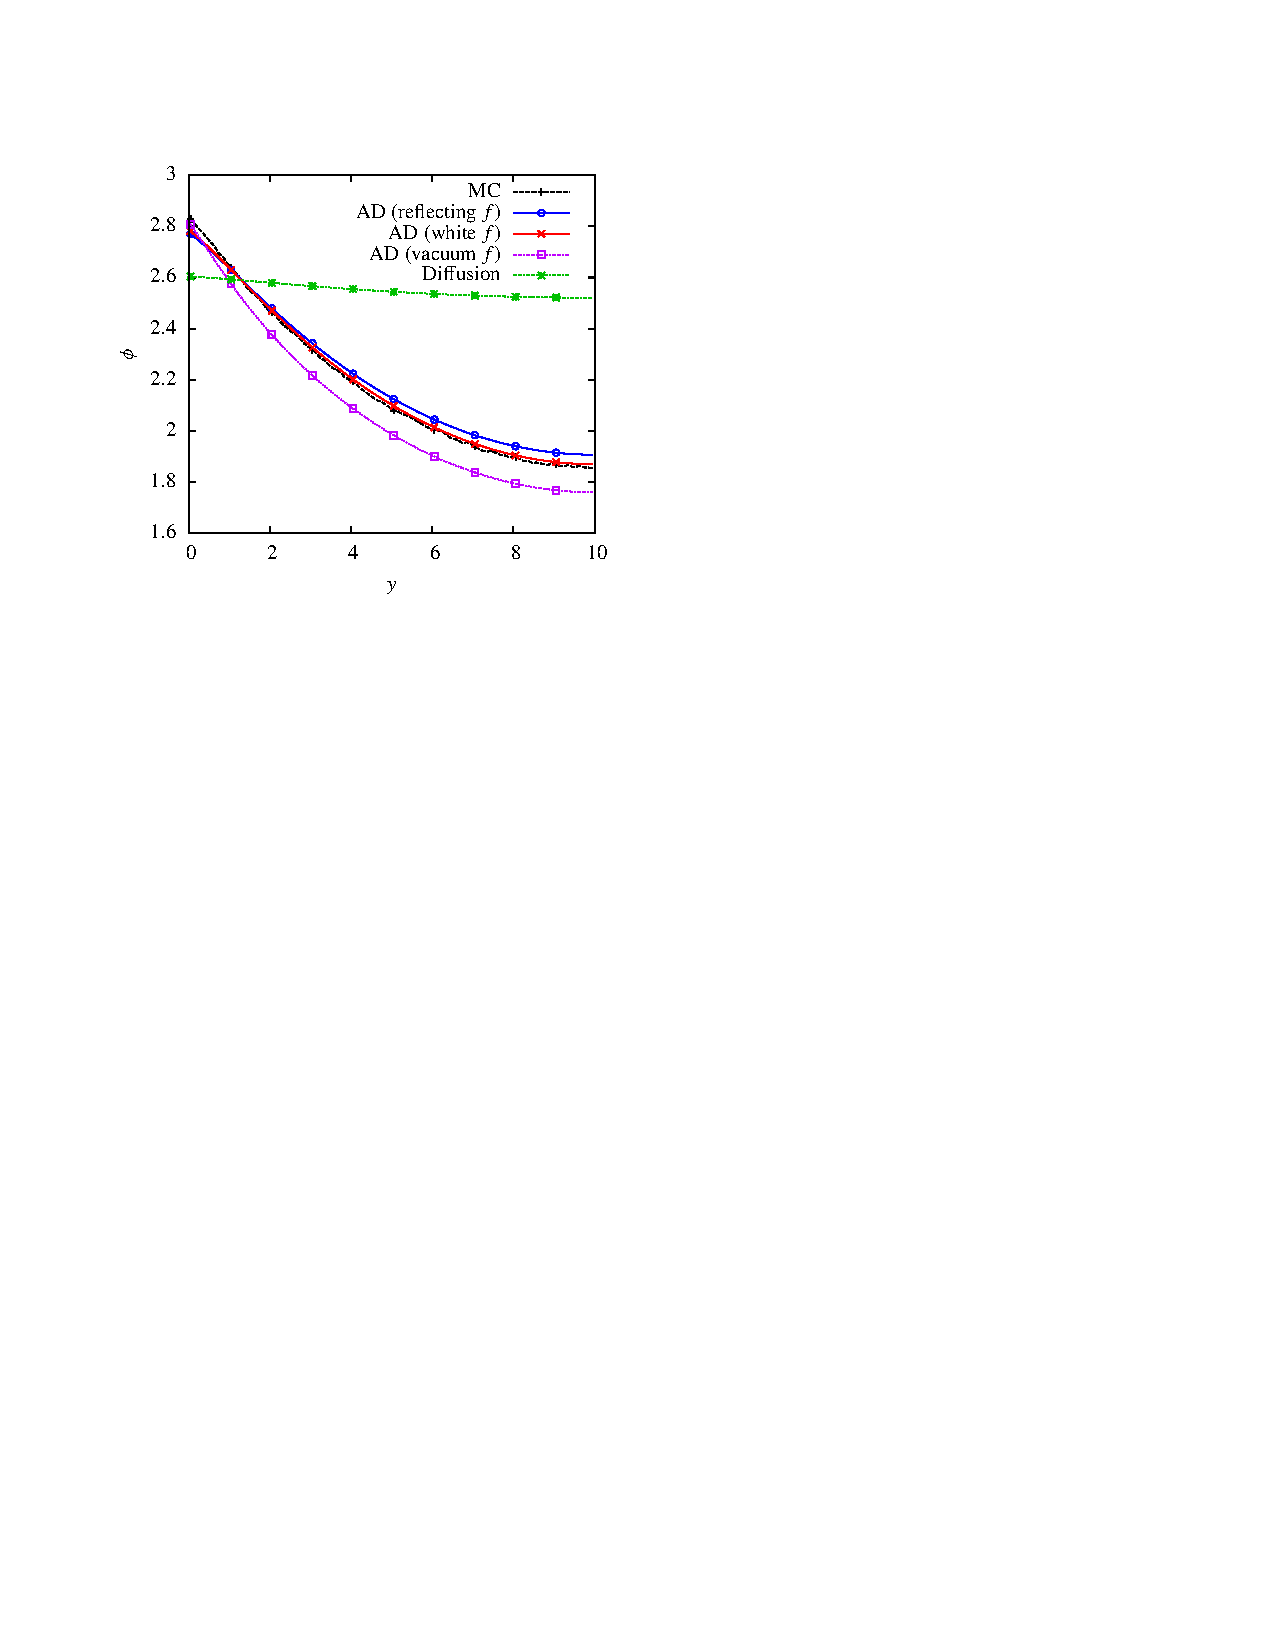
\includegraphics{example_figure}
  \caption{Captions are flush with the left.}
  \label{fig:voltage}
\end{figure}

Later on, we can include a table, even one that spans two columns such as
Table~\ref{tab:widetable}.
%%%%%%%%%%%%%%%%%%%%%%%%%%%%%%%%%%%%%%%%
\begin{table*}[htb]
  \centering
\begin{tabular}{llllllllll}\toprule
      & $\phi_T(0)$      & $\phi_T(10)$      & $\phi_T(20)$      &
      $\phi_D(0)$      & $\phi_D(10)$      & $\phi_D(20)$      & $\rho$      &
      $\varepsilon$      & $N_\text{it}$
\\ \midrule
$c=0.999$  & 0.9038 & 20.63 & 31.24 & 0.9087 & 20.63 & 31.23 & 0.2192 & $10^{-7}$ & 15
\\
$c=0.990$  & 0.3675 & 13.04 & 24.7 & 0.3696 & 13.04 & 24.69 & 0.2184 & $10^{-7}$ & 15
\\
$c=0.900$  & 0.009909 & 4.776 & 17.64 & 0.009984 & 4.786 & 17.63 & 0.2118 & $10^{-7}$ & 14
\\
$c=0.500$  & $6.069\times 10^{-5}$ & 2.212 & 15.53 & 6.213$\times 10^{-5}$ & 2.239 & 15.53 & 0.2068 & $10^{-7}$ & 13
\\
\bottomrule
\end{tabular}
  \caption{This is an example of a really wide table which might not normally
  fit in the document.}
  \label{tab:widetable}
\end{table*}
%%%%%%%%%%%%%%%%%%%%%%%%%%%%%%%%%%%%%%%%
Notice how the table reference uses a Roman numeral
for its numbering scheme, whereas the figure reference uses an Arabic numeral.
For one-column tables, use the \verb|table| environment; two-column tables use
\verb|table*|. The same applies to figures.

%%%%%%%%%%%%%%%%%%%%%%%%%%%%%%%%%%%%%%%%%%%%%%%%%%%%%%%%%%%%%%%%%%%%%%%%%%%%%%%%
\subsection{Another Subsection}
Excessive sectioning in a three-page document is discouraged, but here are more
subsections to demonstrate compliance with the ANS formatting guidelines.

\subsubsection{Third-level Heading}
This subsubsection shows compliance with the ANS-specified standard. This level
of heading should be used rarely.

\subsubsection{Another Such Heading}
And, if you really think you need a third-level heading, you should make sure
that your subsection needs at least two of them.

%%%%%%%%%%%%%%%%%%%%%%%%%%%%%%%%%%%%%%%%%%%%%%%%%%%%%%%%%%%%%%%%%%%%%%%%%%%%%%%%
\section{Conclusions}

The included ANS style file and this clear example file are a panacea for
the hours of headache that invariably results from formatting a document in
Microsoft Word.

%%%%%%%%%%%%%%%%%%%%%%%%%%%%%%%%%%%%%%%%%%%%%%%%%%%%%%%%%%%%%%%%%%%%%%%%%%%%%%%%
\appendix
\section{Appendix}

Numbering in the appendix is different:
\begin{equation} \label{eq:appendix}
  2 + 2 = 5\,.
\end{equation}
and another equation:
\begin{equation} \label{eq:appendix2}
  a + b = c\,.
\end{equation}

%%%%%%%%%%%%%%%%%%%%%%%%%%%%%%%%%%%%%%%%%%%%%%%%%%%%%%%%%%%%%%%%%%%%%%%%%%%%%%%%
\section{Acknowledgments}
This material is based upon work supported a Department of Energy Nuclear
Energy University Programs Graduate Fellowship.

%%%%%%%%%%%%%%%%%%%%%%%%%%%%%%%%%%%%%%%%%%%%%%%%%%%%%%%%%%%%%%%%%%%%%%%%%%%%%%%%
\bibliographystyle{ans}
\bibliography{bibliography}
\end{document}

